\section{Kiến trúc Modular v4.0.0 - Chuyển đổi từ Monolith}

\subsection{Tổng quan về Modular Architecture}

Sự chuyển đổi từ Jupyter Notebook đơn lẻ sang kiến trúc modular đại diện cho một bước nhảy vọt về mặt thiết kế phần mềm. Thay vì tất cả code nằm trong một file, project được tổ chức thành các modules độc lập với trách nhiệm rõ ràng.

\subsection{Data Processing Pipeline và Quy trình Xử lý}

\subsubsection{Tổng quan Pipeline}

AIO Classifier được thiết kế với một data processing pipeline hoàn chỉnh, từ data ingestion đến model deployment. Pipeline này được chia thành các giai đoạn rõ ràng, mỗi giai đoạn tương ứng với một module cụ thể trong kiến trúc.

\begin{table}[H]
\centering
\begin{tabular}{|c|c|c|c|}
\hline
\textbf{Stage} & \textbf{Module} & \textbf{Input} & \textbf{Output} \\
\hline
1. Data Ingestion & \texttt{data\_loader.py} & Dataset paths & Structured data \\
\hline
2. Data Preprocessing & \texttt{wizard\_ui/steps/} & Raw data & Cleaned data \\
\hline
3. Text Vectorization & \texttt{text\_encoders.py} & Text data & Vectorized data \\
\hline
4. Model Training & \texttt{models/} & Vectors & Trained models \\
\hline
5. Model Evaluation & \texttt{comprehensive\_evaluation.py} & Models & Evaluation results \\
\hline
6. Model Deployment & \texttt{app.py} & Models & Web interface \\
\hline
7. Server Training & \texttt{auto\_train.py} & CSV datasets & Automated training \\
\hline
\end{tabular}
\caption{Data Processing Pipeline - Từ Data Ingestion đến Model Deployment}
\label{fig:data_pipeline}
\end{table}

\subsubsection{Chi tiết các Giai đoạn Pipeline}

\textbf{1. Data Ingestion Stage}
\begin{itemize}
    \item \textbf{Module}: \texttt{data\_loader.py}
    \item \textbf{Chức năng}: Tải và quản lý datasets từ nhiều nguồn khác nhau
    \item \textbf{Input}: Dataset paths, configuration parameters
    \item \textbf{Output}: Structured data objects, metadata
    \item \textbf{Features}: 
        \begin{itemize}
            \item Support cho HuggingFace datasets
            \item CSV/JSON file loading
            \item Data validation và type checking
            \item Memory-efficient loading cho large datasets
        \end{itemize}
\end{itemize}

\textbf{2. Data Preprocessing Stage}
\begin{itemize}
    \item \textbf{Module}: \texttt{wizard\_ui/steps/}
    \item \textbf{Chức năng}: Interactive data preprocessing thông qua wizard interface
    \item \textbf{Input}: Raw data từ data ingestion
    \item \textbf{Output}: Cleaned và preprocessed data
    \item \textbf{Features}:
        \begin{itemize}
            \item Column selection và filtering
            \item Data cleaning và validation
            \item Missing value handling
            \item Data type conversion
            \item Real-time preview và validation
        \end{itemize}
\end{itemize}

\textbf{3. Text Vectorization Stage}
\begin{itemize}
    \item \textbf{Module}: \texttt{text\_encoders.py}
    \item \textbf{Chức năng}: Chuyển đổi text data thành numerical vectors
    \item \textbf{Input}: Preprocessed text data
    \item \textbf{Output}: Vectorized data (sparse/dense matrices)
    \item \textbf{Features}:
        \begin{itemize}
            \item Bag of Words (BoW) vectorization
            \item TF-IDF với SVD dimensionality reduction
            \item Word embeddings với GPU acceleration
            \item Intelligent caching system
            \item Memory optimization cho large datasets
        \end{itemize}
\end{itemize}

\textbf{4. Model Training Stage}
\begin{itemize}
    \item \textbf{Module}: \texttt{models/}
    \item \textbf{Chức năng}: Training và optimization của ML models
    \item \textbf{Input}: Vectorized data, training parameters
    \item \textbf{Output}: Trained models, training metrics
    \item \textbf{Features}:
        \begin{itemize}
            \item Multiple model types (KNN, Decision Tree, Naive Bayes, etc.)
            \item GPU acceleration với FAISS
            \item Hyperparameter optimization
            \item Cross-validation và model selection
            \item Ensemble learning capabilities
        \end{itemize}
\end{itemize}

\textbf{5. Model Evaluation Stage}
\begin{itemize}
    \item \textbf{Module}: \texttt{comprehensive\_evaluation.py}
    \item \textbf{Chức năng}: Comprehensive evaluation và comparison của models
    \item \textbf{Input}: Trained models, test data
    \item \textbf{Output}: Evaluation metrics, performance reports
    \item \textbf{Features}:
        \begin{itemize}
            \item Multiple evaluation metrics (accuracy, F1, precision, recall)
            \item Model comparison và ranking
            \item Performance visualization
            \item Statistical significance testing
            \item Export evaluation results
        \end{itemize}
\end{itemize}

\textbf{6. Model Deployment Stage}
\begin{itemize}
    \item \textbf{Module}: \texttt{app.py}
    \item \textbf{Chức năng}: Deployment và serving của trained models
    \item \textbf{Input}: Trained models, user requests
    \item \textbf{Output}: Predictions, model responses
    \item \textbf{Features}:
        \begin{itemize}
            \item Streamlit web interface
            \item Real-time inference
            \item Model versioning và management
            \item User interaction và feedback
            \item Performance monitoring
        \end{itemize}
\end{itemize}

\textbf{7. Server Training Stage}
\begin{itemize}
    \item \textbf{Module}: \texttt{auto\_train.py}
    \item \textbf{Chức năng}: Automated training và deployment của models
    \item \textbf{Input}: CSV datasets, configuration parameters
    \item \textbf{Output}: Trained models, training metrics
\end{itemize}

Để hỗ trợ việc triển khai trên các server environments không phù hợp với giao diện Streamlit, AIO Classifier cung cấp module \texttt{auto\_train.py} - một command-line interface cho phép chạy training tự động mà không cần giao diện web.

\textbf{Mục đích sử dụng:}
\begin{itemize}
    \item \textbf{Server Environments}: Chạy trên các server không có GUI hoặc headless systems
    \item \textbf{Automated Training}: Training tự động với cấu hình pre-defined
    \item \textbf{Batch Processing}: Xử lý hàng loạt datasets mà không cần tương tác người dùng
    \item \textbf{CI/CD Integration}: Tích hợp vào các pipeline tự động hóa
    \item \textbf{Resource Optimization}: Tối ưu hóa tài nguyên server cho training tasks
\end{itemize}

\textbf{Tính năng chính:}
\begin{enumerate}
    \item \textbf{Auto Configuration}: Tự động cấu hình tất cả parameters cần thiết
    \item \textbf{Mode Selection}: Quick Mode (3 models) hoặc Full Mode (4 models)
    \item \textbf{Progress Tracking}: Real-time progress monitoring qua command line
    \item \textbf{Error Handling}: Comprehensive error handling và recovery
    \item \textbf{Result Display}: Detailed results summary sau khi training hoàn thành
    \item \textbf{Cache Management}: Tự động tạo và quản lý cache cho future use
\end{enumerate}

\textbf{Ưu điểm so với Streamlit Interface:}
\begin{itemize}
    \item \textbf{No GUI Required}: Chạy được trên server không có display
    \item \textbf{Lower Resource Usage}: Không cần load web interface
    \item \textbf{Scriptable}: Có thể integrate vào scripts khác
    \item \textbf{Automated}: Không cần user interaction
    \item \textbf{Server-Friendly}: Tối ưu cho production environments
\end{itemize}

\subsubsection{Supporting Modules}

\textbf{Cache System}
\begin{itemize}
    \item \textbf{Module}: \texttt{cache/}
    \item \textbf{Chức năng}: Intelligent caching cho performance optimization
    \item \textbf{Components}:
        \begin{itemize}
            \item \texttt{embeddings/}: Cached word embeddings
            \item \texttt{training\_results/}: Cached model results
            \item \texttt{datasets/}: Cached datasets
        \end{itemize}
\end{itemize}

\textbf{Configuration Management}
\begin{itemize}
    \item \textbf{Module}: \texttt{config.py}
    \item \textbf{Chức năng}: Centralized configuration management
    \item \textbf{Features}:
        \begin{itemize}
            \item Model parameters và hyperparameters
            \item System settings và thresholds
            \item Environment-specific configurations
            \item Runtime parameter adjustment
        \end{itemize}
\end{itemize}

\textbf{Utility Modules}
\begin{itemize}
    \item \textbf{Module}: \texttt{utils/}
    \item \textbf{Chức năng}: Common utilities và helper functions
    \item \textbf{Components}:
        \begin{itemize}
            \item \texttt{progress\_tracker.py}: Progress monitoring
            \item \texttt{rapids\_detector.py}: GPU capability detection
        \end{itemize}
\end{itemize}

\subsubsection{Pipeline Flow Control}

\begin{figure}[H]
\centering
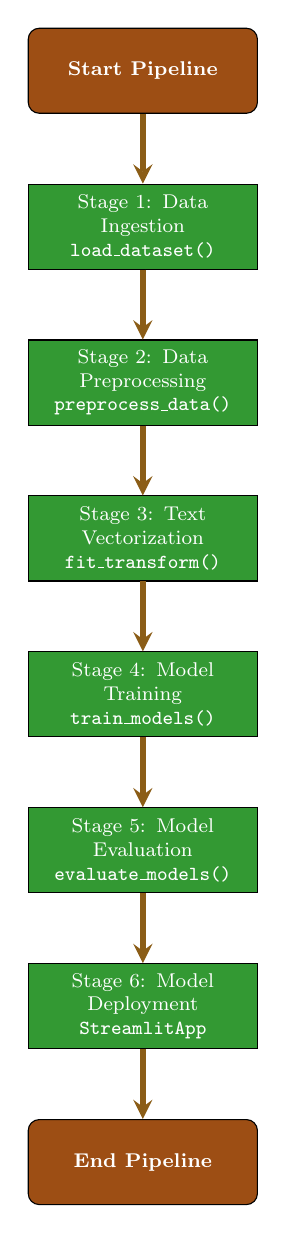
\begin{tikzpicture}[node distance=2.2cm, auto, scale=0.9, transform shape]
    % Define styles with Green-Orange theme
    \tikzstyle{startstop} = [rectangle, rounded corners, minimum width=3.2cm, minimum height=1.2cm, text centered, draw=black, fill={rgb:red,0.8;green,0.4;blue,0.1}, text width=3cm, align=center, font=\footnotesize\bfseries, text=white]
    \tikzstyle{process} = [rectangle, minimum width=3.2cm, minimum height=1.2cm, text centered, draw=black, fill={rgb:red,0.2;green,0.6;blue,0.2}, text width=3cm, align=center, font=\footnotesize, text=white]
    \tikzstyle{arrow} = [thick,->,>=stealth, color={rgb:red,0.6;green,0.4;blue,0.1}, line width=2pt]
    
    % Nodes
    \node (start) [startstop] {Start Pipeline};
    \node (stage1) [process, below of=start] {Stage 1: Data Ingestion\\\texttt{load\_dataset()}};
    \node (stage2) [process, below of=stage1] {Stage 2: Data Preprocessing\\\texttt{preprocess\_data()}};
    \node (stage3) [process, below of=stage2] {Stage 3: Text Vectorization\\\texttt{fit\_transform()}};
    \node (stage4) [process, below of=stage3] {Stage 4: Model Training\\\texttt{train\_models()}};
    \node (stage5) [process, below of=stage4] {Stage 5: Model Evaluation\\\texttt{evaluate\_models()}};
    \node (stage6) [process, below of=stage5] {Stage 6: Model Deployment\\\texttt{StreamlitApp}};
    \node (end) [startstop, below of=stage6] {End Pipeline};
    
    % Arrows
    \draw [arrow] (start) -- (stage1);
    \draw [arrow] (stage1) -- (stage2);
    \draw [arrow] (stage2) -- (stage3);
    \draw [arrow] (stage3) -- (stage4);
    \draw [arrow] (stage4) -- (stage5);
    \draw [arrow] (stage5) -- (stage6);
    \draw [arrow] (stage6) -- (end);
\end{tikzpicture}
\caption{Data Processing Pipeline Flow - Từ Data Ingestion đến Model Deployment}
\label{fig:pipeline_flow}
\end{figure}

\subsubsection{Data Flow và Dependencies}

\begin{figure}[H]
\centering
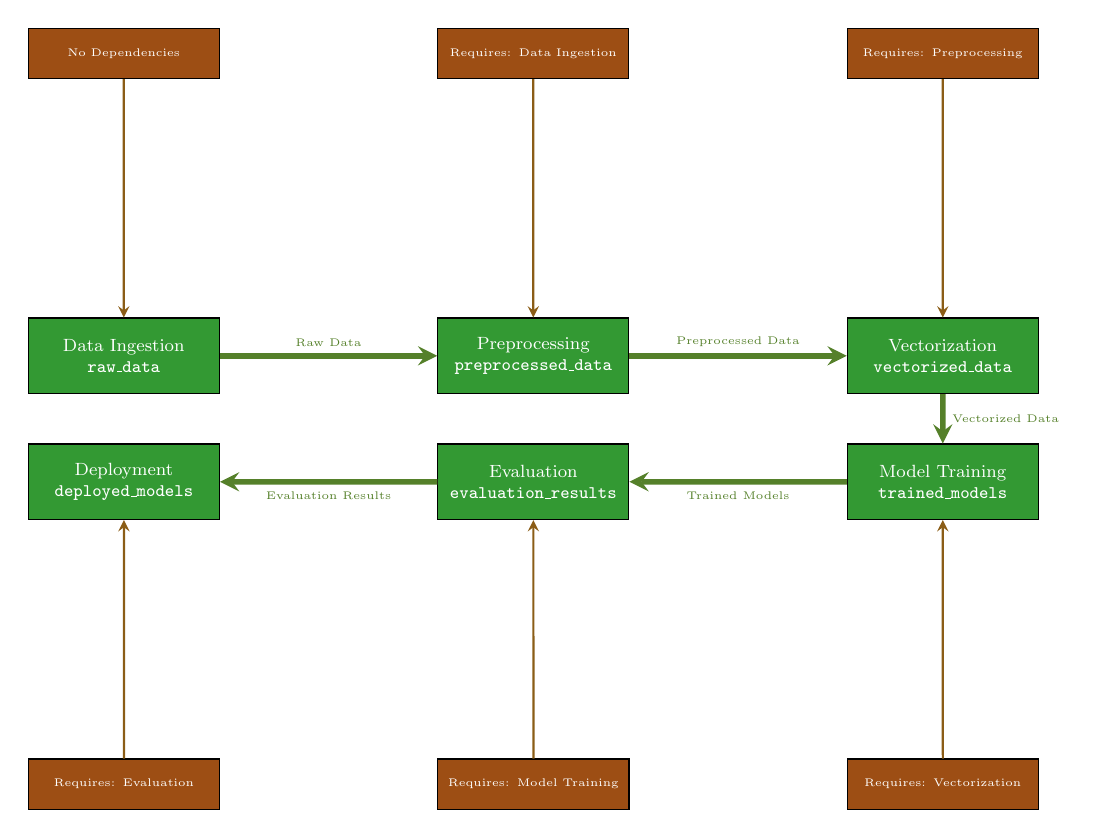
\begin{tikzpicture}[node distance=4cm, auto, scale=0.8, transform shape]
    % Define styles with Green-Orange theme
    \tikzstyle{stage} = [rectangle, minimum width=3cm, minimum height=1.2cm, text centered, draw=black, fill={rgb:red,0.2;green,0.6;blue,0.2}, text width=2.8cm, align=center, font=\footnotesize, text=white]
    \tikzstyle{dependency} = [rectangle, minimum width=3cm, minimum height=0.8cm, text centered, draw=black, fill={rgb:red,0.8;green,0.4;blue,0.1}, text width=2.8cm, align=center, font=\tiny, text=white]
    \tikzstyle{arrow} = [thick,->,>=stealth, color={rgb:red,0.6;green,0.4;blue,0.1}]
    \tikzstyle{dataflow} = [thick,->,>=stealth, color={rgb:red,0.4;green,0.6;blue,0.2}, line width=2pt]
    
    % Main stages - Top row
    \node (stage1) [stage] {Data Ingestion\\\texttt{raw\_data}};
    \node (stage2) [stage, right of=stage1, xshift=2.5cm] {Preprocessing\\\texttt{preprocessed\_data}};
    \node (stage3) [stage, right of=stage2, xshift=2.5cm] {Vectorization\\\texttt{vectorized\_data}};
    
    % Main stages - Bottom row
    \node (stage4) [stage, below of=stage3, yshift=2cm] {Model Training\\\texttt{trained\_models}};
    \node (stage5) [stage, left of=stage4, xshift=-2.5cm] {Evaluation\\\texttt{evaluation\_results}};
    \node (stage6) [stage, left of=stage5, xshift=-2.5cm] {Deployment\\\texttt{deployed\_models}};
    
    % Dependencies - Top row
    \node (dep1) [dependency, above of=stage1, yshift=0.8cm] {No Dependencies};
    \node (dep2) [dependency, above of=stage2, yshift=0.8cm] {Requires: Data Ingestion};
    \node (dep3) [dependency, above of=stage3, yshift=0.8cm] {Requires: Preprocessing};
    
    % Dependencies - Bottom row
    \node (dep4) [dependency, below of=stage4, yshift=-0.8cm] {Requires: Vectorization};
    \node (dep5) [dependency, below of=stage5, yshift=-0.8cm] {Requires: Model Training};
    \node (dep6) [dependency, below of=stage6, yshift=-0.8cm] {Requires: Evaluation};
    
    % Data flow arrows - Top row
    \draw [dataflow] (stage1) -- node[above, font=\tiny] {Raw Data} (stage2);
    \draw [dataflow] (stage2) -- node[above, font=\tiny] {Preprocessed Data} (stage3);
    
    % Data flow arrows - Top to Bottom
    \draw [dataflow] (stage3) -- node[right, font=\tiny] {Vectorized Data} (stage4);
    
    % Data flow arrows - Bottom row
    \draw [dataflow] (stage4) -- node[below, font=\tiny] {Trained Models} (stage5);
    \draw [dataflow] (stage5) -- node[below, font=\tiny] {Evaluation Results} (stage6);
    
    % Dependency arrows - Top row
    \draw [arrow] (dep1) -- (stage1);
    \draw [arrow] (dep2) -- (stage2);
    \draw [arrow] (dep3) -- (stage3);
    
    % Dependency arrows - Bottom row
    \draw [arrow] (dep4) -- (stage4);
    \draw [arrow] (dep5) -- (stage5);
    \draw [arrow] (dep6) -- (stage6);
\end{tikzpicture}
\caption{Data Flow và Dependencies giữa các Pipeline Stages}
\label{fig:data_flow_dependencies}
\end{figure}

\subsection{Cấu trúc thư mục mới}

\begin{minted}{bash}
models/
├── __init__.py              # Package initialization
├── base/                    # Base classes và interfaces
│   ├── base_model.py        # Abstract base class
│   ├── interfaces.py        # Protocol definitions
│   └── metrics.py           # Common evaluation metrics
├── clustering/              # Clustering models
│   └── kmeans_model.py      # K-Means implementation
├── classification/          # Classification models
│   ├── knn_model.py         # K-Nearest Neighbors
│   ├── decision_tree_model.py
│   ├── naive_bayes_model.py
│   ├── logistic_regression_model.py
│   ├── linear_svc_model.py
│   └── svm_model.py
├── ensemble/                # Ensemble learning
│   ├── ensemble_manager.py
│   └── stacking_classifier.py
├── utils/                   # Utility modules
│   ├── model_factory.py     # Factory pattern
│   ├── model_registry.py    # Model registration
│   └── validation_manager.py
└── new_model_trainer.py     # Advanced trainer
\end{minted}

\subsection{Cross-Validation và Hyperparameter Tuning}

\paragraph{Advanced Model Trainer với Cross-Validation}

\texttt{AdvancedModelTrainer} là một component quan trọng trong kiến trúc AIO Classifier, được thiết kế để thực hiện training models với các kỹ thuật tiên tiến như cross-validation và hyperparameter tuning. Class này cung cấp các phương thức để đánh giá hiệu suất model một cách toàn diện và phát hiện overfitting.

\textbf{Các tính năng chính:}

\begin{itemize}
    \item \textbf{Cross-Validation Training}: Sử dụng k-fold cross-validation để đánh giá model một cách khách quan và đáng tin cậy
    \item \textbf{Multi-Metric Evaluation}: Đánh giá model trên nhiều metrics đồng thời (accuracy, precision, recall, F1-score)
    \item \textbf{Overfitting Detection}: Tự động phát hiện overfitting bằng cách so sánh training score và validation score
    \item \textbf{Statistical Analysis}: Cung cấp mean và standard deviation của các metrics để đánh giá độ ổn định
    \item \textbf{Factory Integration}: Tích hợp với ModelFactory để tạo và quản lý các model instances
\end{itemize}

\textbf{Quy trình hoạt động:}

\begin{enumerate}
    \item \textbf{Model Creation}: Tạo model instance thông qua ModelFactory dựa trên model name
    \item \textbf{Scoring Configuration}: Định nghĩa các scoring metrics cần đánh giá
    \item \textbf{Cross-Validation Execution}: Thực hiện k-fold cross-validation với dataset
    \item \textbf{Overfitting Analysis}: Tính toán và phân tích overfitting score
    \item \textbf{Results Compilation}: Tổng hợp kết quả và trả về comprehensive evaluation report
\end{enumerate}

\textbf{Lợi ích của Advanced Model Trainer:}

\begin{itemize}
    \item \textbf{Reliable Evaluation}: Cross-validation đảm bảo đánh giá khách quan, không bị bias
    \item \textbf{Overfitting Prevention}: Tự động phát hiện và cảnh báo khi model bị overfitting
    \item \textbf{Performance Insights}: Cung cấp insights chi tiết về hiệu suất và độ ổn định của model
    \item \textbf{Automated Workflow}: Tự động hóa quá trình training và evaluation
    \item \textbf{Scalable Design}: Có thể dễ dàng mở rộng để hỗ trợ thêm các kỹ thuật evaluation khác
\end{itemize}

\subsection{So sánh với Notebook ban đầu}

\begin{table}[H]
\centering
\begin{tabular}{|l|c|c|}
\hline
\textbf{Aspect} & \textbf{Notebook} & \textbf{Modular} \\
\hline
Code Organization & Monolithic & Modular \\
\hline
Number of Models & 3 & 7+ \\
\hline
Error Handling & Basic & Comprehensive \\
\hline
Extensibility & Limited & High \\
\hline
Testing & Manual & Automated \\
\hline
Documentation & Comments & Full docs \\
\hline
Performance & Basic & Optimized \\
\hline
Maintainability & Low & High \\
\hline
\end{tabular}
\caption{So sánh Notebook vs Modular Architecture}
\end{table}

\subsection{Ưu điểm của Modular Architecture}

\begin{enumerate}
    \item \textbf{Scalability}: Dễ dàng thêm models và features mới
    \item \textbf{Maintainability}: Code được tổ chức rõ ràng, dễ maintain
    \item \textbf{Testability}: Mỗi component có thể test độc lập
    \item \textbf{Reusability}: Components có thể reuse trong projects khác
    \item \textbf{Type Safety}: Type hints và interfaces rõ ràng
    \item \textbf{Performance}: Optimized cho large datasets
    \item \textbf{Error Handling}: Comprehensive error handling và logging
\end{enumerate}

\subsection{Nhược điểm và Trade-offs}

\begin{enumerate}
    \item \textbf{Complexity}: Code phức tạp hơn, khó hiểu cho beginners
    \item \textbf{Overhead}: Có overhead từ abstraction layers
    \item \textbf{Learning Curve}: Cần hiểu design patterns
    \item \textbf{File Count}: Nhiều files hơn, có thể confusing
\end{enumerate}

\subsection{Kết luận}

Kiến trúc Modular đại diện cho một bước tiến quan trọng trong việc phát triển ML applications. Mặc dù phức tạp hơn notebook ban đầu, nó cung cấp foundation vững chắc cho việc phát triển production-ready systems với khả năng mở rộng và maintainability cao.
